\lstset{inputpath = ../MATLAB}
\graphicspath{{./figures/chapter4/}}

\chapter{Source code} \label{ch:appendix-source-code}

The final version of the code comprises 2500 lines of vectorized MATLAB code and
1600 lines of C++ code, excluding comments and empty lines
but including some extra numerical simulations and mesh generation programs
not shown in this work.

MATLAB was chosen for the implementation of high-level routines like
the Runge-Kutta methods and the finite volume schemes because
of its interactive environment, which makes it very suitable for
quick numerical experiments, whereas a compiled language like C++
was chosen for the implementation of the most performance-sensitive
parts of the code (the reconstruction routines) because of its speed.
The C++ functions are connected to MATLAB through the MEX interface,
which makes it possible for the two languages to share the same data
structures in memory.

The LAPACK library is used for the linear algebra routines related to
QR decomposition and the solution of least squares problems.
The OpenMP programming interface is used to speed up
the C++ code even further by computing the reconstructions on the
boundary of each cell in parallel.
The output of every simulation is saved in a sequence of .vtk files
that can be read by Paraview, an open-source data analysis and visualization
application widely used in fluid dynamics for post-processing tasks.

More or less every numerical routine references three fundamental data structures
named \texttt{vertices}, \texttt{edges} and \texttt{cells}.
In addition to the geometrical description of the mesh over which the partial
differential equation is discretized, these structures contain all the quantities
required by the finite volume method such as the cell averages $\bar{\vec{u}}_i$,
the numerical fluxes, and the reconstructions $\vec{u}_{ijk}^+$, $\vec{u}_{ijk}^-$.
The fields of these data structures, being a sort of mutual agreement between
all the different pieces of code involved, are carefully documented in the
following text file. \\

\lstinputlisting[label=prog:polymesh-FVM-txt,language={},
caption={Documentation of the most important data structures.},
linerange=4-114]{FVM Solver/polymesh_FVM.txt}
\vspace{1em}

\lstinputlisting[label=prog:polymesh-FVM-header-geometry,language=C++,
caption={C++ header of \texttt{vertices}, \texttt{edges} and \texttt{cells};
geometrical data}]{Geometry/polymesh.h}
\vspace{1em}

\lstinputlisting[label=prog:polymesh-FVM-header-FVM,language=C++,
caption={C++ header of \texttt{vertices}, \texttt{edges} and \texttt{cells};
FVM data}]{FVM Solver/polymesh_FVM.h}
\vspace{1em}

\lstinputlisting[label=prog:solver,inputencoding=utf8/latin1,
caption={Main loop of the numerical simulation.}]{FVM Solver/solver.m}
\vspace{1em}

\lstinputlisting[label=prog:FVM-initialize, inputencoding=utf8/latin1,
caption={Initialization of the Finite Volume Method.}]{FVM Solver/FVM_initialize.m}
\vspace{1em}

\lstinputlisting[label=prog:vtk-from-polymesh-bin, inputencoding=utf8/latin1,
caption={Code that saves the current state of the simulation in a .vtk file.}]
{Euler Equation/vtk_from_polymesh_bin.m}
\vspace{1em}

\lstinputlisting[label=prog:SSPRK11, caption={Strong Stability Preserving
Runge-Kutta method, order 1.}]{FVM Solver/SSPRK11.m}
\vspace{1em}

\lstinputlisting[label=prog:SSPRK22, caption={Strong Stability Preserving
Runge-Kutta method, order 2.}]{FVM Solver/SSPRK22.m}
\vspace{1em}

\lstinputlisting[label=prog:SSPRK33, caption={Strong Stability Preserving
Runge-Kutta method, order 3.}]{FVM Solver/SSPRK33.m}
\vspace{1em}

\lstinputlisting[label=prog:FVM,inputencoding=utf8/latin1,
caption={Finite Volume Method.}]{FVM Solver/FVM.m}
\vspace{1em}

\lstinputlisting[label=prog:check-state2D,inputencoding=utf8/latin1,
caption={Check if the values $\bar{\vec{u}}_i$ are admissible in every cell.}]
{Euler Equation/check_state2D.m}
\vspace{1em}

\lstinputlisting[label=prog:check-edges-state2D,inputencoding=utf8/latin1,
caption={Check if the values $\vec{u}^+$ and $\vec{u}^-$ are admissible
on every edge.}]{FVM Solver/check_edges_state2D.m}
\vspace{1em}

\lstinputlisting[label=prog:numerical-flux-rusanov,
caption={Rusanov's numerical flux.}]{FVM Solver/numerical_flux_rusanov.m}
\vspace{1em}

\lstinputlisting[label=prog:max-wave-speed-2D,
caption={Max wave speed 2D.}]{Euler Equation/max_wave_speed2D.m}
\vspace{1em}

\lstinputlisting[label=prog:reconstruction-LLS1,language=C++,
caption={Constant reconstructions (order 1).}]
{FVM Solver/reconstruction_LLS1.cpp}
\vspace{1em}

\lstinputlisting[label=prog:method,language=C++,
caption={C++ header of \texttt{method}.}]{FVM Solver/method.h}
\vspace{1em}

\lstinputlisting[label=prog:reconstruction-LLS2,language=C++,
caption={Linear Least Squares reconstruction of order 2.}]
{FVM Solver/reconstruction_LLS2.cpp}
\vspace{1em}

\lstinputlisting[label=prog:reconstruction-LLS3,language=C++,
caption={Linear Least Squares reconstruction of order 3.}]
{FVM Solver/reconstruction_LLS3.cpp}
\vspace{1em}

\lstinputlisting[label=prog:reconstruction,language=C++,inputencoding=utf8/latin1,
caption={C++ code used to build stencils and solve least squares problems.}]
{FVM Solver/reconstruction.h}
\vspace{1em}

\lstinputlisting[label=prog:reconstruction-T1WENO,language=C++,
caption={Type-I WENO reconstruction of order up to 3.}]
{FVM Solver/reconstruction_T1WENO.cpp}

\lstinputlisting[label=prog:vortex,inputencoding=utf8/latin1,
language=MATLAB,caption={Isentropic vortex.}]{Simulation Entropy Vortex/vortex.m}
\vspace{1em}

%\begin{figure}[p]
%\centering
%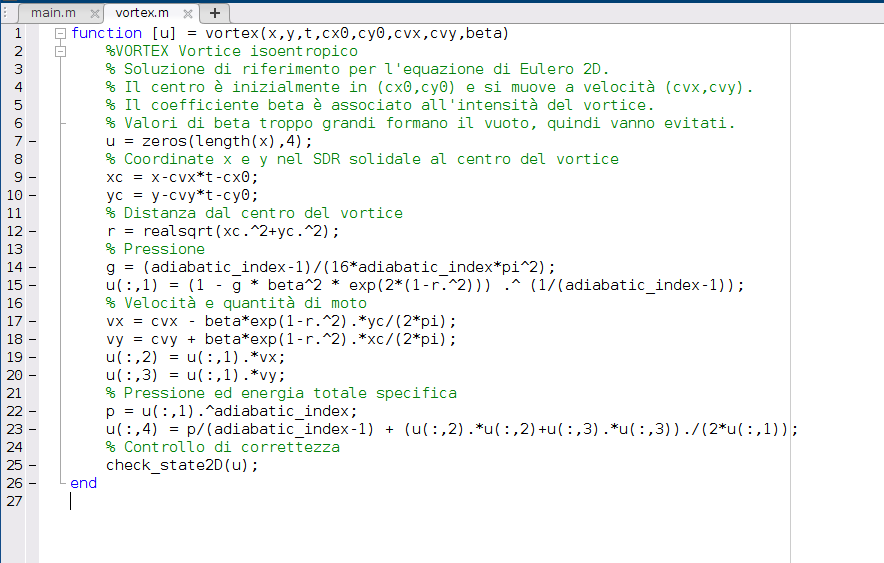
\includegraphics[scale=0.5]{foobar.png}
%\caption{Isentropic vortex.}
%\label{prog:vortex}
%\end{figure}





